% !Mode:: "TeX:UTF-8"

\chapter{超像素分割和图像分割理论基础}

本文第1章介绍了超像素和图像分割的基本概念,并分类介绍了超像素分割和图像分割的研究背景及研究现状。
在本章中将对相关的基本理论进行简要的介绍。
首先简要叙述深度学习和神经网络的相关理论研究,接着介绍经典的基于神经网络的图像分割方法。
然后简述超像素的两个经典算法以及超像素在图像分割的意义。此外,介绍了将超像素整合到神经网络中的理论基础-超像素池化层。

\section{深度学习}
\begin{figure*}[h]
\begin{center}
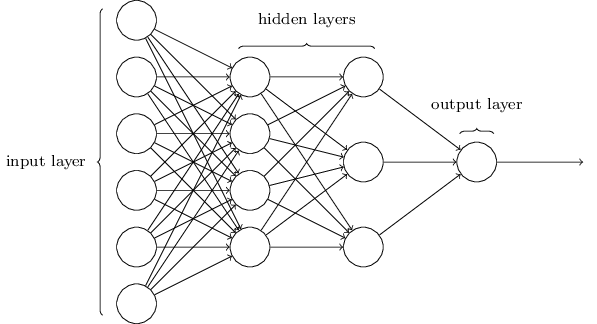
\includegraphics[width=1\textwidth]{figures/CNN0.png}
\end{center}
\vspace{-5mm}
\caption{多层感知器示意图}
\label{fig2.1}
\end{figure*}
%概念,分类,
2016年3月,在中央发表的"十三五"规划纲要中,“人工智能”一词格外引人注目。
BAT等各大互联网公司对人工智能领域的投入更是将人工智能这一领域的发展推向一个新的高潮。
目前深度学习\cite{2006DL}无疑是人工智能的重点研究领域之一,设计到人工智能众多领域,如计算机视觉、自然语言处理等。

%浅层区别  《深度学习研究综述》
深度学习其实是机器学习的一种,从最初的浅层机器学习发展到目前深度学习。与浅层机器学习相比,深度学习加深了模型结构深度,一般有5 层,6 层,甚至更多的隐层节点。
一般而言,随着深度的增加,模型的学习能力也在增加。
此外,深度学习是一种特征学习,能够利用大数据来学习特征,从而能够获取数据更高层次的抽象表示,来描述数据的内在信息。

深度学习的概念源于人工神经网络的研究,深度学习网络最基本的结构是多层感知器(multilayer perception,MLP)。多层感知器,也就是我们所说的前向传播网络,一般有多层构成,每一层由若干神经元组成,如图\ref{fig2.1}所示。



如图\ref{fig2.2}所示,对于第$l$层,多层感知器的前向传播公式如下:
\begin{equation}
y_{i}^{k+1} = \sum_{j}W_{k}^{ij}y_{j}^{k}+b_{i}^{k}
\end{equation}
其中,$y_{j}^{k}$表示第$k$层的第$j$个神经元的输出,
$W_{k}^{ij}$表示第$k$层中第$j$个神经元与第$k+1$层的第$i$个神经元之间的权重,$b_{i}^{k}$是偏置值。
通常进行完这一步之后,会在此基础上使用非线性激活函数进行激活运算,常见的激活函数有ReLU、Sigmoid等。

\begin{figure*}[h]
\begin{center}
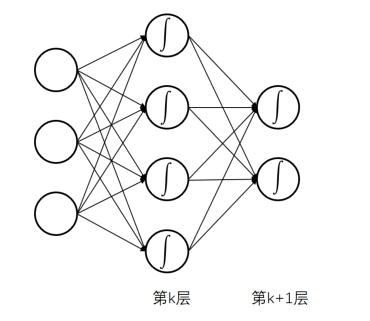
\includegraphics[width=0.8\textwidth]{figures/CNN01.png}
\end{center}
\vspace{-5mm}
\caption{前向传播示意图}
\label{fig2.2}
\end{figure*}
%应用
由于理论和计算力的原因,深度学习从提出到本世纪出,深度学习一度被边缘化,成果泛善可陈,直到2012年ImageNet比赛,多伦多大学团队开发的AlexNet\cite{2012AlexNet}模型的出现,以卷积神经网络(Convolutional Neural Network,CNN)\cite{krizhevsky2012imagenet}为基础,识别效果超过了所有浅层的方法。从此开启了深度学习进入快速发展的新时期,已经被广泛应用到计算机视觉、语言识别、自然语言处理等领域。

2015年的世界大规模人脸识别竞赛LFW中,来着香港中文大学多媒体实验室的中国团队使用深度学习模型,打败FaceBook团队获得冠军。使得在人脸识别领域,深度学习的识别能力穿越真人。
此外在计算机视觉领域中的行人检测、多人姿态估计、物体跟踪、场景识别、图像分类、图像分割、物体跟踪等都有深度学习的身影。
近年来,科研人员也将深度学习应用到很多有意思的方向,例如:去除马赛克、风格迁移、黑白照片自动上色、图片补全等。

深度学习虽然很早应用于计算机视觉,但在语音处理领域最先取得突破性进展。语音处理主要分为语音识别和语音合成两大方向。2016 年,微软利用深度学习开发的语言识别模型,在日常对话识别准确度上首先达到了人类水平,真正让大家大吃一惊。此外,各大公司也都在研究利用深度学习来进行语言合成,并已有成熟的系统,例如谷歌的WaveNet模型,百度的Deep Voice3。

2013年,Tomas Mikolov等人发表论文《Efficient Estimation of Word Representations in Vector Space》\cite{2013word2vector},提出了word2vector 模型,这也是目前自然语言处理通常使用的模型,与传统的词袋模型(bag of words)相比,word2vector能够更好地表达语法信息。
目前深度学习在自然语言处理领域的应用主要包括:问答系统、情感分析、机器翻译、句子成分分析等。
\section{卷积神经网络}

%定义
简单来说,卷积神经网络(Convolutional Neural Network,CNN)是深度学习模型中的其中一类,类似于人工神经网络的多层感知器。
Yann LeCun提出的LeNet\cite{1998Gradient}模型,最早将CNN应用于数字识别。2012年,多伦多大学Alex Krizhevsky等人开发的AlexNet\cite{2012AlexNet}模型第一次让大家注意到了CNN的强大之处。

% 网络结构
LeNet模型只有卷积层和池化层,全连接层,后来AlexNet模型在此基础上,加入了Relu激励层,提高了效率。接下来会分别介绍相关理论和计算。

% 卷积操作
\begin{figure*}[h]
\begin{center}
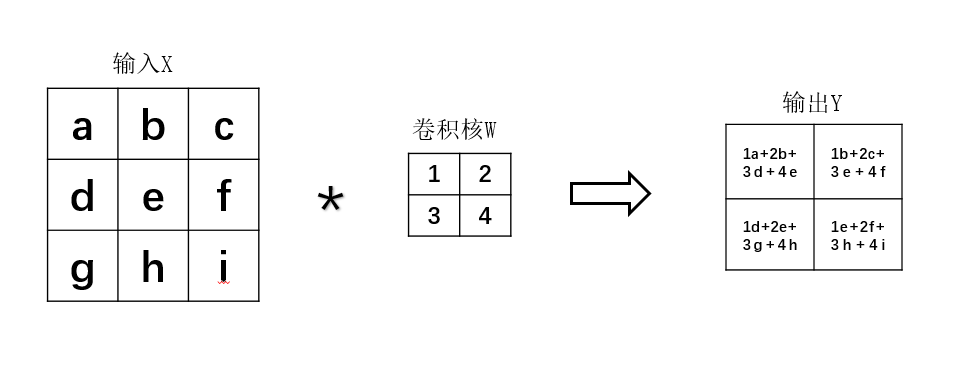
\includegraphics[width=1\textwidth]{figures/CNN1.png}
\end{center}
\vspace{-5mm}
\caption{卷积计算过程示意图}
\label{fig2.3}
\end{figure*}

卷积层作为卷积神经网络最重要的一层,其作用主要是提取图像的局部特征。如图\ref{fig2.3}所示,卷积层的卷积操作为卷积核W 与输入矩阵X 进行从左到右从上到下,步长为1的相乘相加操作,得出输出Y。卷积核W的大小为$M_w \times N_w$,输入矩阵的大小为$M_x \times N_x$, 那么输出矩阵的大小等于$(M_x-M_w+1)\times(N_x-N_w+1)$。
以图\ref{fig2.4}为例,一个$3\times 3$的卷积核在一个$5\times 5$的输入图像上以步长为1做卷积计算,
得到$3\times 3$的输出矩阵,这个输出矩阵就是特征矩阵。

\begin{figure*}[h]
\begin{center}
%\fbox{\rule{0pt}{2in} \rule{.9\linewidth}{0pt}}
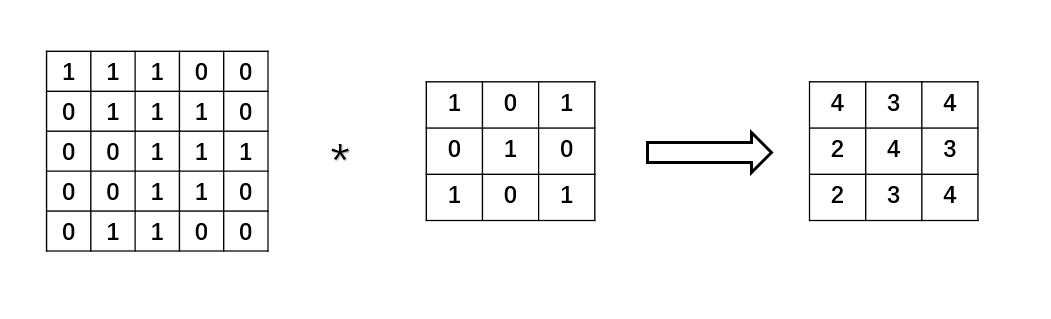
\includegraphics[width=1\textwidth]{figures/CNN2.png}
\end{center}
\vspace{-5mm}
\caption{卷积操作示意图}
\label{fig2.4}
\end{figure*}

%Relu激活
最原始的感知机(perceptron)并没有激活层,无论有多少层神经网络,输出层的结都是输入数据的线性组合,不能满足解决神经网络复杂任务的需求。因而加入了激活层,使用非线性函数作为激活函数,使得深层神经网络有了学习的能力,可以逼近任何函数。

用sigmoid函数和tanh函数作为最初的激活函数,输出有界,很容易充当下一层的输入。
随着神经网络的深度增加,卷积神经网络在反向传播过程中存在梯度消失的问题,
Sigmoid等激活函数的导数很小,而连续多个很小的数相乘,结果几乎为0,因此梯度无法从输出层传到输入层。随着神经网络的深度增加会造成梯度消失的问题,从而导致训练难度大,效果不佳。此外,反向传播求梯度时,Sigmoid函数计算量较大。

2012年提出的AlexNet引入了一种新的激活函数-ReLU函数。该函数的提出很大程度的解决了深层神经网络的梯度耗散问题,而且减少了计算量。此外,ReLU会使一部分神经元的输出为0,这样就造成了网络的稀疏性,并且减少了参数的相互依存关系,缓解了过拟合问题的发生。

现在也有一些对ReLU的改进,比如prelu,random ReLU等,对于不同的任务上,准确率或速度上有一定的改进。
此外,现在卷积神经网络,一般会在ReLU激活层之后会多做一步归一化操作,尽可能保证每一层网络的输入具有相同的分布,减少计算量。

% 池化操作
在连续的卷积层之间一般会放入池化层,其目的是压缩数据,降低维度,减少计算。
池化层用的方法包括最大池化(Max Pooling)和平均池化(Average Pooling)。以最大池化为例,如图\ref{fig2.5}所示,在一个$4\times4$ 的矩阵上,选用$2\times2$的filters,步长为2,对于每个$2\times 2$ 的窗口选出最大的数作为输出矩阵的相应元素的值,比如输入矩阵第一个$2\times 2$窗口中最大的数是6,那么输出矩阵的第一个元素就是6,如此类推。平均池化的原理类似,只不过输出矩阵中的元素是输入矩阵对应窗口中元素的平均值。
\begin{figure*}[h]
\begin{center}
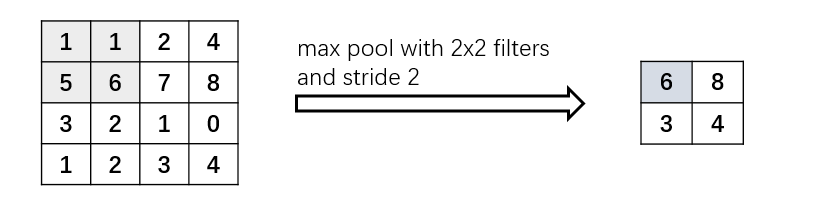
\includegraphics[width=1\textwidth]{figures/CNN3.png}
\end{center}
\vspace{-5mm}
\caption{池化操作示意图}
\label{fig2.5}
\end{figure*}

接下来具体介绍池化层的具体作用。如果输入数据是一张图片,那么池化层的作用就是对图像进行压缩。压缩过程中,去掉一些无关紧要的特征信息,留下最能体现图像特征的信息。我们知道,一张图像中含有的很多的信息,也具有很多的特征,但是有些特征信息,对于需要完成的任务则显得无关紧要,过于冗余。池化操作就是要去除这些冗余信息,留下最重要的特征信息。

池化操作具有特征不变性。所谓的特征不变性就是一张狗的图像被缩小了一倍,但还能认出这是一张狗的照片。
这说明在压缩过程中只是去除了无关紧要的信息,但对狗的重要特征信息仍有保留,因此我们依然可以能判断出这是一只狗。
% 发展

批归一化(Batch Normalization,BN)\cite{ioffe2015batch}是深度学习发展中的一个里程碑式的技术,使各种网络能够进行训练。
在卷积神经网络训练过程中,由于参数是不断更新的,随着网络层数的加深,对于深层网络,其输入数值不稳定,导致模型很难收敛。通过归一化,对中间层的输出结果进行标准化处理,使得其更加稳定,分布更加固定,有利于算法的稳定和收敛。

然而,沿着批处理维度进行规范化会带来问题——当批处理大小变小时,BN的错误会迅速增加,这是由于批次统计估计不准确造成的。2018年,Yuxin Wu提出了组归一化(Group Normalization,GN)\cite{wu2018group},GN将通道分成组,并计算每组中的均值和方差进行归一化。GN的计算与批量大小无关,更适合于批次较小的任务。

\section{基于卷积神经网络的图像分割}
%《基于深度学习的RGB-D图像语义分割》
%《FCN》http://www.sjocr.com/news/915.html
上文介绍了卷积神经网络的概念以及相关理论基础,CNN相对传统算法而言,其最大的优点在于通过构造神经网络,可以自动学习到不同层次的特征。
浅层网络具有较小的感受野,可以学习到包含更多细节信息的局部特征。
深层网络具有更大的感受野,学习到的特征更加抽象,包含更多的全局特征。
这些全局特性相对来说更加笼统,对物体的颜色、大小、位置等信息敏感性更低,对于分类更有帮助,可能更加方便的辨别出物体的类别。
但是由于缺失了细节信息,不能精确的给出图像中的像素属于哪个物体,因而给不出物体的精确轮廓,做不到准备的分割效果。

传统基于卷积神经网络的方法为了确定某个像素所属的类别,从而实现图像分割,一般将该像素周围的像素块作为卷积神经网络的输入来进行训练。
这样造成了几个缺点:
一是增加了存储开销,例如对于每个像素分类任务,采用的像素块为$15\times 15$,其需要原来的225倍的存储空间。
二是对在相邻像素块进行运算,由于相邻像素块的重叠,其大部分运算是重复的,无用的,导致计算效率降低。
三是像素块相对于整个图像而言小很多,在卷积神经网络训练中,对像素块进行卷积提取特征,只能提取到局部信息,导致分类的性能有所限制。

Long等人提出了全卷积网络(Fully Convolutional Network,FCN)\cite{long2015fully} 解决了以上问题,成功应用于图像分割。
与经典的CNN在卷积层使用全连接层得到固定长度的特征向量进行分类不同,FCN可以接受任意尺寸的输入图像,采用反卷积层对最后一个卷积层的特征图进行上采样,使它恢复到与输入图像相同的尺寸,从而可以对每一个像素都产生一个预测,同时保留了原始输入图像中的空间信息,最后基于在上采样的特征图进行像素的分类。

\begin{figure*}[h]
\begin{center}
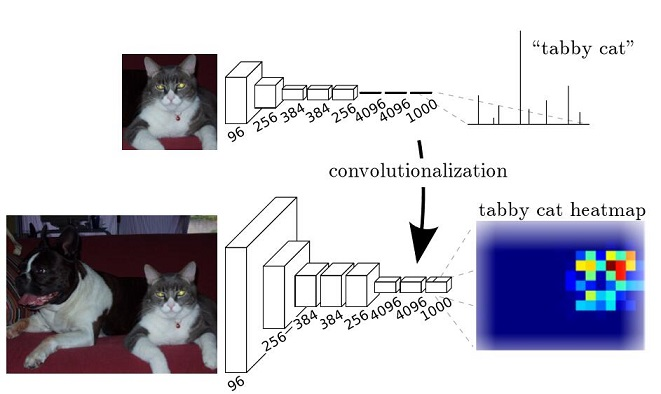
\includegraphics[width=1\textwidth]{figures/FCN1.jpg}
\end{center}
\vspace{-5mm}
\caption{FCN网络流程图}
\label{fig2.6}
\end{figure*}

如图\ref{fig2.6}所示,FCN将传统卷积神经网络中最后三层的全连接层全都换成卷积层。
传统卷积神经网络中,经过最后三层的全连接层分别会得到长度为4096、4096、1000的一维向量。
FCN使用卷积核大小分别为(4096,1,1)、(4096,1,1)、(1000,1,1)的卷积层替换全连接层。

经过前五层的卷积和池化操作,图像大小变成了原图像的1/2、1/4、1/8、1/16、1/32,分辨率逐渐降低。
为了恢复图像的分辨率,FCN采用了反卷积进行上采样操作,例如对第五层的结果进行反卷积,放大32倍,恢复到原图大小。

但由于深层特征缺失细节信息,得到的结果并不准确。FCN创造性的采用了跳层连接操作。
如图\ref{fig2.7}所示,第二层卷积池化之后,图像变为原图大小的1/4,从第三层卷积池化之后,保存池化后的输出。
经过五层的卷积池化,分别得到原图的1/8、1/16、1/32大小的特征图。
然后对第五层输出(即1/32尺寸的特征图)进行反卷积,上采样之后结果和第四层输出进入相加求和,从而补充细节信息,得到16 倍上采样结果。
同样,其结果继续和第三层输出进行求和相加,继续补充细节信息,得到8倍上采样结果。
最终使得结果越来越精确。

FCN可以输入任意大小的图像,不再像以往的卷积神经网络对训练图像和测试图像的大小有限制。虽然经过跳层连接,进行了补充细节信息,但是得到的结果不是很精确。此外,没有充分考虑像素与像素之间的关系,忽略了局部信息的关联性。

\begin{figure*}[h]
\begin{center}
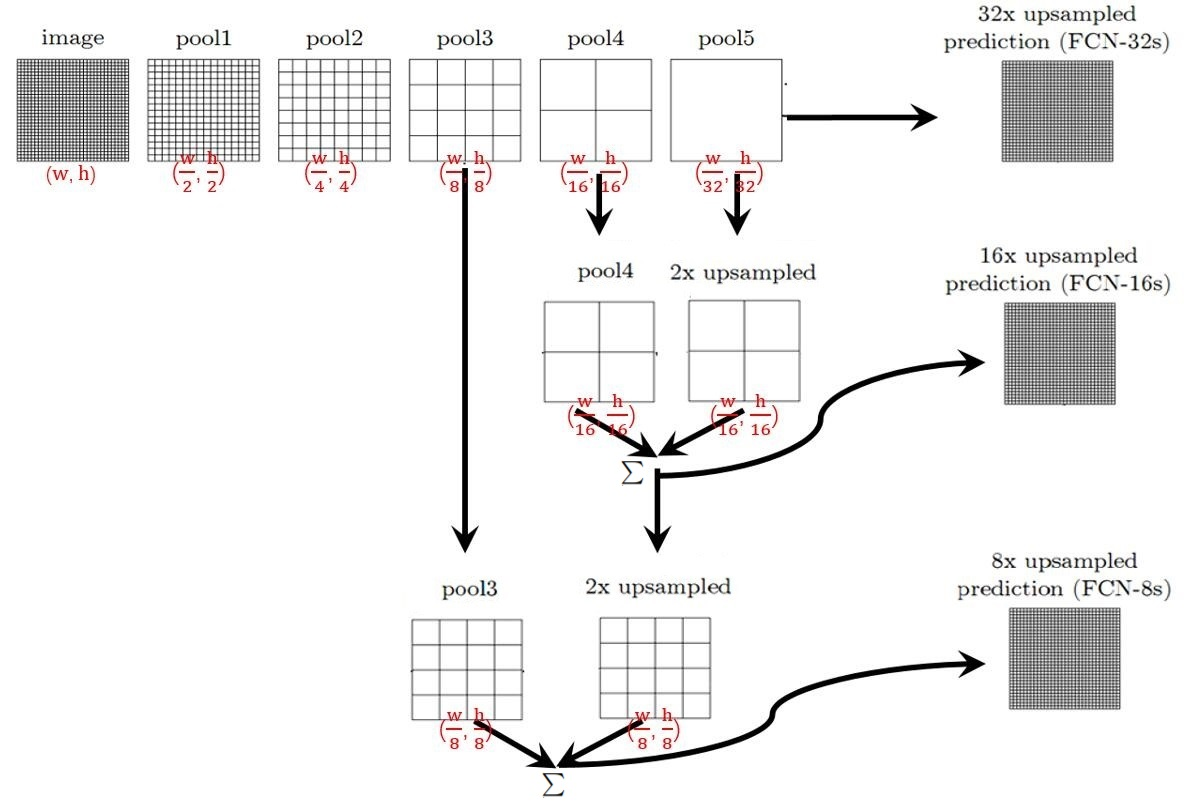
\includegraphics[width=1\textwidth]{figures/FCN2.jpg}
\end{center}
\vspace{-5mm}
\caption{跳层连接结构示意图}
\label{fig2.7}
\end{figure*}

\section{超像素分割算法以及超像素在图像分割中的意义}

\subsection{SLIC超像素分割}

SLIC作为最经典的超像素分割算法,具有很多优点,
计算简单且速度快,可以生成规则的超像素,此外可以控制超像素数量。但是其
生成的超像素边界的保持效果并不理想,而且抗噪性较差。SLIC将彩色图像转
换为CIELAB颜色空间和XY坐标系下的5维特征向量,然后构造5维特征向量的
距离度量来对像素进行局部聚类。这个想法简单易行。与其他超像素分割方法相
比,SLIC算法在速度、紧凑性等方面都是理想的。

其具体实现步骤包括:

1.初始化种子中心:通过设置超像素的个数,实现在图像内均匀分配种子点。例如一张图像具有$N$个像素,划分为$M$个超像素,则每个超像素中像素数目为$N/M$,相邻种子点的距离为$S=\sqrt{N/M}$。

2.局部区域重新确定种子中心:为了避免初始种子中心落在区域边缘上,从而影响聚类结果。需要在初始种子点的$n\times n$邻域(一般设为n=3),计算所有像素点的梯度,选择梯度值最小的点作为种子点。

3. 为像素点分配种子标签:对于每个像素点,在$2S\times 2S$的区域内搜索种子点,进行距离度量,选取最小值对应的种子点作为该像素的聚类中心,从而来分配种子标签,得到K个超像素。
距离度量由颜色距离和空间距离构成。

颜色距离计算公式为:
\begin{equation}
d_c=\sqrt{\left ( l_j-l_i\right )^{2}+\left ( a_j-a_i\right )^{2}+\left ( b_j-b_i\right )^{2}}
\end{equation}

空间距离计算公式为:
\begin{equation}
d_s=\sqrt{\left ( x_j-x_i\right )^{2}+\left ( y_j-y_i\right )^{2}}
\end{equation}

距离度量公式为:
\begin{equation}
D = \sqrt{\left ( \frac{d_c}{N_c}\right )^{2}+\left ( \frac{d_s}{N_s}\right )^{2}}
\end{equation}
其中$N_c$代表最大颜色距离,一般设为常数。$N_s=S=\sqrt{N/M}$。

4. 更新聚类中心:
计算这$K$个聚簇里所有像素点的平均向量值,重新得到$K$个聚类中心。
然后以这$K$个中心,再计算与其周围$2S\times 2S$区域内的像素距离度量,从而分配新的种子标签。
更新聚类中心,再次迭代,如此反复直到收敛。

5. 增加连通性:避免出现超像素过小、孤立点的情况。

\subsection{基于图的超像素分割}
%https://wenku.baidu.com/view/4f5c813cfe4733687e21aab2.html
基于图像法的基本思想是将图像中的像素映射成加权无向图,
无向图中的一个顶点代表了图像中的一个像素,点与点之间边的权重由像素之间的特性差异性计算得来。
基于图论法就是将加权无向图根据一定的准则划分为数个连通子树,从而得到超像素分割结果。

Felzenszwalb和Huttenlocher提出了一种基于图的快速高效分割方法FH\cite{felzenszwalb2004efficient},
将像素作为无向图的顶点,利用边缘权重用于测量顶点之间的不相似性。
类似于其他区域合并方法,它使用Kruskal\cite{2003Boruvka}算法来构建最小生成树,其中每棵树都是一个超像素区域。
每个顶点最初都放置在其自己的组件中,并且FH方法通过这样的准则合并区域,即所产生的分割既不会太粗糙也不会太精细。
FH方法基于图像相邻区域中的可变性程度来自适应地调整分割标准,从而即使做出贪婪的决策,它也服从某些全局属性。
%然而,如最近的研究[9],[10]所示,分割不足的误差很高。

其思路是将图像映射到无向图$G=(V,E)$。$G=(V,E)$表示由$n$个顶点$v\in V$和$m$个边$e\in E\subseteq V\times V$。
每个像素与一个顶点相关联,并与它的4个邻域局部连接。
每个边$e_{ij}=(v_i,v_j)$都被分配了一个权重(通常为非负实值),该权重度量两个顶点$v_i$和$v_j$之间的差异。
分割区域S是将图G划分为数个不相交的分量,每个小区域$C\in S$对应一个连通子图${G}'=({V}',{E}')$,
其中${V}'\subseteq V$和${E}'\subseteq E$。

该方法将区域C对应的最小生成树MST(C,E)中的最大权重作为区域C的内部差异,其计算公式为:
\begin{equation}
Int(C) = \max_{e\in MST(C,E)}W(e)
\end{equation}

将连接两个区域的最小权重边作为它们之间的区域差异性,其表示为:
\begin{equation}
Dif(C_1,C_2)=\min_{v_i\in C_1,v_j\in C_2,(v_i,v_j)\in E}W((v_i,v_j))
\end{equation}

通过比较两个区域的区域差异性和它们的内部差异来判断是否进行合并。
若区域差异性大于它们之间任意一个的内部差异,则不能进行合并,可以用下面公式来表明:
\begin{equation}
D(C_1,C_2)=
\left\{\begin{matrix}
false & if & Dif(C_1,C_2)> MInt(C_1,C_2) \\
true & \text{otherwise}
\end{matrix}\right.
\end{equation}

其中,$MInt(C_1,C_2)=min(Int(C_1)+\tau(C_1),Int(C_2)+\tau(C_2))$。通过$\tau(C)= = \frac{k}{\left | C\right |}$,来控制两个区域的差异性,保证区域差异性一定大于两个区域的内部差异性。k为设定的常数,$\left | C\right |$ 为区域C中顶点的个数,即像素的个数。

2018年,Xing Wei等人提出Superpixel Hierarchy,利用Boruvka算法实现无向图的区域合并。
本文在第4章详细介绍了过程。
其优点是具有线性时间解,可并行化。此外,该方法在聚类的过程中融入了
局部信息,比SLIC和LSC等只利用每像素特征来确定聚类隶属关系的方法更为健壮。

接下来,本文详细比较了Boruvka算法和Kruskal算法各自的特性以及优缺点。

\subsection{Kruskal算法 VS Boruvka算法}

基于图论的分割算法,其基本思路是将图像映射到加权无向图中,利用最小生成树算法对无向图进行分割。
最经典也最常用的算法有Kruskal算法和Boruvka算法。

Kruskal算法构造最小生成树的主要思想是:
假设无向图$G=(V,E)$由$n$个顶点$v\in V$和$m$个边$e\in E\subseteq V\times V$组成。
初始状态下,每个顶点可以看成一个连通分量。
选取E中权值最小的边$e$,若边$e$的两个顶点属于同一个连通分量,则舍去继续寻找并判断下一条权重最小的边。
若$e$的两个顶点属于不同的连通分量,则利用边$e$将两个连通分量合并在一起。
以此类推,经过数次迭代,直达所有顶点在同一连通分量,这个连通分量便是无向图$G$的最小生成子树。

Kruskal算法最重要的是在构建连通分量过程中考虑是否会形成环的情况。
当选取了权重最小的边,若这条边连接了不同的连通分量,说明这两个连通分量加入这条边之后,不会构成环路,
从而可以将这个边连接的连通分量合并在一起。
如这条边的两个顶点在同一个连通分量中,加入这条边之后必然产生环路,故而应该舍去这条边。

其算法步骤为:
\begin{itemize}
\item 步骤1: 初始状态下无向图$G=(V,E)$由$n$个顶点$v\in V$和$m$个边$e\in E\subseteq V\times V$组成,每个顶点看成一个连通分量。
\item 步骤2: 计算所有边的权重,并将所有边根据权重进行从小到大的排序。
\item 步骤3: 选择权重最小的边,判断其两端的顶点是否在同一连通分量中。
两个顶点若属于不同的连通分量,则利用此边将两个连通分量合并。
若两个顶点属于同一个的连通分量,则舍弃此边。
\item 步骤4: 重复步骤3,直到所有顶点在同一个连通分量为止。
\end{itemize}

Boruvka算法基本思想从当前所有的连通分量向外拓展,取最小边向其他连通块进行连接,直到只剩一个连通块。它是基于Kruskal算法和Prim算法。取最小边的贪心思想是 Kruskal的算法主体;向外扩展,连接其他连通分量又是Prim的思想。

Prim算法即从图中的某一顶点出发,计算与其连接的各个边的权重,选取权重最小的边,连接那个顶点。
继而计算这两个顶点相邻的所有顶点,同样与权重最小的边所连接的顶点进行连接。以此类推,直到连接所有的顶点。
在拓展连接其他连通分量时,同Boruvka算法一样,也需要进行是否会形成环的判断。
Boruvka算法相对于Boruvka算法最大的优点是可以并行化,具有线性时间解。

其算法步骤为:
\begin{itemize}
\item 步骤1: 初始状态下无向图$G=(V,E)$由$n$个顶点$v\in V$和$m$个边$e\in E\subseteq V\times V$组成,每个顶点看成一个连通分量。
\item 步骤2: 对于每个连通分量,计算并寻找与其相邻的最小权重边。
\item 步骤3: 对找到的边与对应的连通分量,进行是否构成环路的判断。
若不构成环路,则此边连接的顶点加入到对应的连通分量中。
否则舍弃此边。
\item 步骤4: 重复步骤2和步骤3,直到所有顶点在同一个连通分量为止。
\end{itemize}


\subsection{超像素在图像分割中的意义}
%《基于图论的超像素分割及合并算法》
对于图像分割任务,基于像素的传统处理方法取得了不错的成果。
但是随着数码产品的拍照功能迅速发展,图像的构成越来越复杂,分辨率不断增大,越来越清晰,包括的像素数量也是成指数级增长。
在这样的背景下,基于像素的传统图像分割方法处理分辨率高的图像,将花费更多的时间。

如何减少图像分割的计算量显得尤为重要。超像素作为一种图像预处理技术解决了这个问题。
所谓超像素,就是由局部的许多像素构成的区域,这些区域内的像素通常由具有相似纹理、颜色、亮度等特征。
相对于像素而言,超像素不仅有效减少了局部的冗余信息,后续处理过程中的计算量和复杂度大幅度降低,而且更利于局部特征的提取与表达,更有利于帮助定位区域的边界。

\section{超像素池化层}

2017年,Suha Kwak等人提出了Superpixel Pooling Network (SPN)\cite{kwak2017weakly}网络,将超像素分割结果作为低阶结构的表征,利用提出的超像素池化层对输入网络的超像素进行提取特征,辅助语义分割的推断。
此外,SPN网络验证了使用了超像素对于提高图像分割的准确率,确实能起到一定的效果。

在这里简单介绍一下SPN网络中超像素池化层的具体操作,每个超像素的特征向量生成如公式\ref{eq2.8}所示:
假设 $P_{i}= \left \{ p_{i}^{k} \right \} k=1,2,\cdots ,K_i$ 。$P_{i}$表示图像中
第$i $个超像素,$K_i$表示第$i$个超像素中像素的个数,对于每个超像素$P_{i}$,
超像素特征的计算公式为:

\begin{equation}
v_{i} = \frac{1}{K_i}\sum_{j}\sum_{k}I(p_{i}^{k}\in r^{j})z^{j}
\label{eq2.8}
\end{equation}
其中,$r^{j}$表示感受野, $z^{j}$表示经过上采样得到的特征图中的第j个位置的值。 $I(p_{i}^{k}\in r^{j})$是一个indicator 函数,如果括号中的值为true,则返回1,否则返回0。

固定当前某一个超像素,将之池化。式中的$r$存在是因为存在尺度差异,是感受野大小。
作者的池化方式是固定超像素,遍历特征图和超像素内的元素,计算当前超像素元素在位置j感受野所占的比例,然后加权上去。
通过式\ref{eq2.8}便可以得到每个超像素的特征向量,从而可进行后续的运算。

\section{本章小结}

本章主要介绍了超像素分割和图像分割理论基础以及相关算法。
首先分别深度学习的相关知识,包括深度学习的概念与发展,多层感受器,深度学习在计算机视觉与自然语言处理中的应用。
然后详细介绍了卷积神经网络的各个基础组件,这也是本文构建的神经网络的基础。以LeNet模型和AlexNet模型为例,介绍了卷积神经网络的卷积层,激活层,池化层以及激活层。
在第2.3小结,以FCN为例,详细介绍了卷积神经网络在图像分割领域的应用。
2.4小结中,首先介绍了超像素分割的经典算法-SLIC算法和基于图论的相关算法。然后介绍了对比了基于图论的两个基础算法-Kruskal算法和Boruvka算法。最后说明了超像素在图像分割中的意义。
最后一节中,介绍了超像素池化层,将超像素引入神经网络提供了理论基础以及实现的可能。
